%I wrote this from scratch because every time I'd download a template and change anything it would break everything.

%Compiled with the atom 'latex' package.
%atom 'language-latex' package for syntax highlighting.
%atom 'pdf-view-plus' to compile and immediately see changes in atom.

%COMPILE WITH THIS COMMAND WHICH I MADE A BASH ALIAS FOR. NO HASSLE COMPILATION THIS IS LIKE A GOLDEN EGG.
%alias texcomp="lualatex -interaction nonstopmode $1"
%────────────────────────────────────────────────────────────────────────────────────────────────────────────────────────────────
%\documentclass[12pt]{article}
%\pagestyle{plain}

\documentclass{article}
\usepackage[english]{babel}
%\usepackage[utf8]{inputenc}
\usepackage{fancyhdr}

%Reference pics from images subfolder.
\usepackage{graphicx}
\graphicspath{ {./images/} } %dir of embedded images, less clutter in main dir.

\usepackage{lipsum}
\usepackage[margin=20mm]{geometry} %Set margins
\usepackage{setspace}
\renewcommand{\baselinestretch}{1} %Change between pacing between elements.

\usepackage{amsmath}
\numberwithin{equation}{section}
%───────────────────────────────────────────────────────────────────────────────────────────────────────────────────────────────

                                                  %────────────────┐
                                                  \begin{document}%│
                                                  %────────────────┘
%────────────────────────────────────────────────────────────────────────────────────────────────────────────────────────────────
%Page header and footer
\pagestyle{fancy}
\fancyhf{}
\rhead{Owen Fitzgerald - Fall 2020}
\lhead{Class}
\rfoot{Page \thepage}
%────────────────────────────────────────────────────────────────────────────────────────────────────────────────────────────────
%Homework info
\begin{center}
  {\LARGE\textbf{Homework Template}} \\
  {\large\emph{\textbf{Chapter x}}}
\end{center}

\begin{flushleft}

  {\textbf{Student:} {\emph{Owen Fitzgerald}}} \\
  {\textbf{Due Date: } {\emph{TBD}}} \\
  {\textbf{Professor:} {\emph{Dr. Ward}}} \\
  {\LaTeX\textbf{ Path:} {\emph{\textasciitilde/Documents/school/template.tex}}} \\

  \noindent\makebox[\linewidth]{\rule{\linewidth}{.4pt}}

\end{flushleft}
%────────────────────────────────────────────────────────────────────────────────────────────────────────────────────────────────

%QUESTIONS
\noindent\makebox[\linewidth]{\rule{\linewidth}{1pt}}
%────────────────────────────────────────────────────────────────────────────────────────────────────────────────────────────────
\section{Question 1}
\emph{\lipsum[2]}\\

  \subsection*{\emph{Solution}}
    \begin{center}

        {\begin{equation} F(x) &= \int^a_b \frac{1}{3}x^3 \end{equation}} \\
        {\begin{equation} \left(\frac{1}{\sqrt{x}}\right) \end{equation}} \\
        {\begin{equation} \left\frac{1}{x}\right \end{equation}} \\


    \end{center}

\noindent\makebox[\linewidth]{\rule{\linewidth}{1pt}}
%────────────────────────────────────────────────────────────────────────────────────────────────────────────────────────────────	-
\section{Question 2}
\emph{\lipsum[1]}\\

  \subsection*{\emph{Solution}}
    \begin{center}

      {\begin{equation} F(x) &= \int^a_b \frac{1}{3}x^3 \end{equation}} \\
      {\begin{equation} \left(\frac{1}{\sqrt{x}}\right) \end{equation}} \\
      {\begin{equation} \left\frac{1}{x}\right \end{equation}} \\

    \end{center}

\noindent\makebox[\linewidth]{\rule{\linewidth}{1pt}}
%────────────────────────────────────────────────────────────────────────────────────────────────────────────────────────────────

%────────────────────────────────────────────────────────────────────────────────────────────────────────────────────────────────
\section{Figure}
\emph{\lipsum[3]}\\

  \begin{figure}[h!]
  \begin{center}

    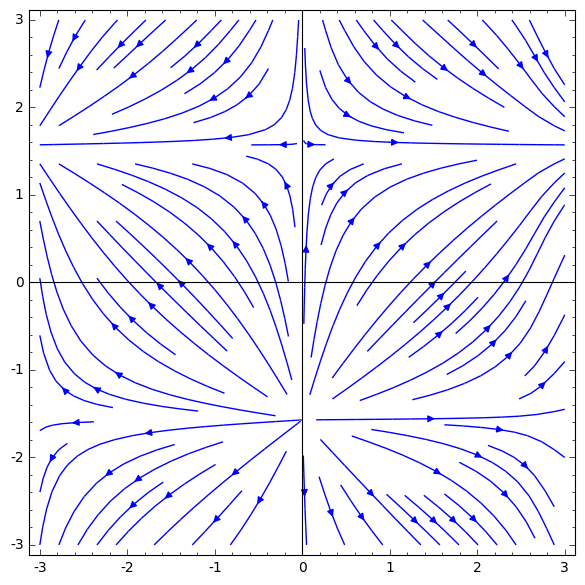
\includegraphics[scale=.75]{plot_5}
    \caption{Example figure}

    \label{fig:atom}
  \end{center}
  \end{figure}

%────────────────────────────────────────────────────────────────────────────────────────────────────────────────────────────────
\end{document}
